% ============================================================
% NC-SLU: Sub-100K On-Device SLU with Few-Shot Intent Addition
% Target: EMNLP 2026 via ARR (May 25, 2026 deadline)
% ============================================================
\documentclass[11pt]{article}
\usepackage{acl}
\usepackage[T1]{fontenc}
\usepackage{amsmath,amssymb}
\usepackage{booktabs}
\usepackage{multirow}
\usepackage{graphicx}
\usepackage{xcolor}
\usepackage{tikz}
\usetikzlibrary{positioning,arrows.meta,fit,calc}
\usepackage{algorithm}
\usepackage{algorithmic}

\definecolor{ncblue}{HTML}{1A73E8}
\definecolor{ncgreen}{HTML}{34A853}
\definecolor{ncred}{HTML}{EA4335}

\title{NC-SLU: On-Device Spoken Language Understanding \\ in Sub-100K Parameters with Few-Shot Intent Addition}

\author{Jin Ho Choi \\
  NanoAgentic AI / SmartEar Inc. \\
  Seoul, South Korea \\
  \texttt{jhchoi@nanoagentic.ai}}

\begin{document}
\maketitle

% ============================================================
% ABSTRACT
% ============================================================
\begin{abstract}
Spoken language understanding (SLU) systems typically rely on large pre-trained models with millions of parameters, making on-device deployment impractical for battery-constrained edge devices.
We present \textbf{NC-SLU}, the first sub-100K parameter end-to-end SLU system capable of few-shot intent addition without full retraining.
NC-SLU systematically compares four backbone variants---NC-TCN, NC-TCN-Bi, NC-SSM, and NC-SSM-Bi (21K--26K parameters)---evaluating causal vs.\ bidirectional temporal modeling with convolution and state-space architectures for intent classification.
We introduce \textbf{NC-OPAL} (Neural-Compressed Online Prototype Adaptation with LoRA), a two-stage incremental learning method combining prototype-imprinted heads, low-rank adaptation ($r{=}2$), and knowledge distillation ($\lambda_{\text{KD}}{=}5$) to add new intents from as few as 20 examples while preserving base intent accuracy.
On the Fluent Speech Commands benchmark (31 intents), NC-SLU achieves \textbf{TBD\%} overall accuracy with 25 base intents and 6 new intents added via 20-shot learning.
On the incremental KWS benchmark (GSC V2, 35 keywords), NC-OPAL achieves \textbf{85.76\%} ACC---within 3.75\%p of methods using 3$\times$ more parameters.
NC-SLU enables real-time intent classification on microcontrollers with sub-256KB memory.
Code is available at \url{https://github.com/DrJinHoChoi/NC-KWS-FineTuning}.
\end{abstract}

% ============================================================
% 1. INTRODUCTION
% ============================================================
\section{Introduction}

Spoken language understanding (SLU)---mapping speech directly to semantic intents---is a critical component of voice-controlled edge devices such as smart home controllers, hearing aids, industrial HMIs, and wearable AI assistants.
The dominant paradigm cascades an automatic speech recognition (ASR) module with a natural language understanding (NLU) module, or employs large end-to-end models pre-trained on massive speech corpora \cite{lugosch2019speech,arora2023espnetslu,radford2023whisper}.

While effective, these approaches face fundamental deployment constraints on edge devices:
\begin{itemize}
\setlength\itemsep{1pt}
\item \textbf{Model size}: Pre-trained SLU models (e.g., ESPnet-SLU with HuBERT) require 90M+ parameters (360MB+), far exceeding MCU memory limits (256KB--2MB).
\item \textbf{Computation}: Real-time inference requires sub-10ms latency, ruling out transformer-based architectures on resource-constrained hardware \cite{banbury2021mlperf}.
\item \textbf{Adaptability}: Deploying new intents (``turn on the fan'') typically requires full retraining with all data, impractical for personalized on-device customization.
\end{itemize}

We ask: \emph{Can a model with fewer than 100K parameters perform end-to-end SLU with the ability to add new intents from minimal examples?}

We answer affirmatively with \textbf{NC-SLU}, which makes three contributions:

\begin{enumerate}
\setlength\itemsep{1pt}
\item \textbf{Ultra-compact SLU with backbone comparison}: We systematically compare four sub-100K backbones---NC-TCN, NC-TCN-Bi, NC-SSM, NC-SSM-Bi---for end-to-end SLU on Fluent Speech Commands \cite{lugosch2019speech}, achieving competitive accuracy at $\sim$\textbf{4,000$\times$ fewer parameters} than ESPnet-SLU.

\item \textbf{NC-OPAL}: A two-stage incremental learning method---prototype-imprinted head initialization followed by LoRA fine-tuning with knowledge distillation---that adds new intents from 20 examples per class while limiting catastrophic forgetting.
On the incremental KWS benchmark (GSC V2), NC-OPAL achieves 85.76\% ACC with 21K parameters, within 3.75\%p of methods using 3$\times$ more parameters.

\item \textbf{First sub-100K incremental SLU}: To our knowledge, this is the first demonstration of class-incremental spoken language understanding at the sub-100K parameter scale, bridging the gap between on-device keyword spotting and full SLU systems.
\end{enumerate}

% ============================================================
% 2. RELATED WORK
% ============================================================
\section{Related Work}

\paragraph{End-to-End SLU.}
\citet{lugosch2019speech} pioneered E2E SLU by pre-training on word-level labels before fine-tuning for intent classification on Fluent Speech Commands (FSC), achieving 98.8\% accuracy with $\sim$2M parameters.
ESPnet-SLU \cite{arora2023espnetslu} provides a comprehensive toolkit built on large pre-trained encoders (HuBERT, wav2vec2.0) exceeding 90M parameters.
The SLURP benchmark \cite{bastianelli2020slurp} extends SLU evaluation with 72K recordings across 18 domains.
All existing E2E SLU systems require at minimum hundreds of thousands of parameters.

\paragraph{On-Device Speech Understanding.}
SpeechCache \cite{benazir2024speechcache} achieves on-device SLU on MCU-class hardware (STM32, 2MB memory) via a learning cache with 0.5M parameters (1.8MB footprint), resolving 45--90\% of inputs locally.
TinyS2I \cite{tinys2i2022} classifies frequent utterances on-device and defers unsupported ones to the cloud.
For keyword spotting (KWS), sub-100K models are well-studied: BC-ResNet \cite{kim2021bcresnet}, TC-ResNet \cite{choi2019temporal}, and SSM-based architectures \cite{gu2024mamba}.
However, none of these compact models address the richer intent semantics required for SLU.
Our NC-SLU achieves SLU with 21K--26K parameters---\textbf{23$\times$ smaller} than SpeechCache.

\paragraph{Few-Shot Intent Detection.}
\citet{mittal2020fewshot} proposed representation-based meta-learning for few-shot spoken intent recognition, achieving 78.5\% on FSC with 5-shot learning.
In the NLP domain, few-shot intent detection from text has been explored \cite{zhang2020fewshot,xia2021incremental}, and prototypical networks \cite{snell2017prototypical} offer a natural framework.
However, no prior work combines few-shot intent addition with an ultra-compact ($<$100K) speech model that can run on microcontrollers.

\paragraph{Class-Incremental Learning.}
CIL addresses adding new classes without forgetting old ones \cite{rebuffi2017icarl,masana2022class}.
\citet{paul2022incremental} studied class-incremental intent classification for NLP with BERT, finding knowledge distillation most effective.
In speech, DE-KWS \cite{dekws2025} and AnalyticKWS \cite{analytickws2025} demonstrate CIL for keyword spotting---AnalyticKWS achieves 89.51\% on GSC-v2 (6 tasks) with TC-ResNet-8 and single-epoch adaptation.
Our NC-OPAL extends CIL to SLU by combining prototype imprinting, LoRA \cite{hu2022lora}, and knowledge distillation \cite{hinton2015distilling} in a unified framework for sub-100K models.

% ============================================================
% 3. METHOD
% ============================================================
\section{Method}

\subsection{Problem Formulation}

We define on-device incremental SLU as follows.
Given a base set of $C_0$ intents with full training data, the model must:
(1)~learn to classify speech utterances into these intents;
(2)~incrementally add $C_{\text{new}}$ intents using only $K$ examples per class ($K$-shot);
(3)~maintain accuracy on all previously learned intents.

Formally, at time $t$, the model $f_\theta$ maps speech waveform $\mathbf{x} \in \mathbb{R}^{T}$ to an intent label $y \in \{1, \ldots, C_0 + C_{\text{new}}\}$.

\subsection{Ultra-Compact Backbone Architectures}

All four backbones share a common noise-conditioned (NC) front-end: STFT $\rightarrow$ SNR estimation $\rightarrow$ Learned Spectral Gate $\rightarrow$ DualPCEN $\rightarrow$ InstanceNorm $\rightarrow$ Patch Projection.
The backends differ only in their temporal modeling:

\paragraph{NC-TCN (22,411 params at 31 classes).}
Causal dilated temporal convolution with gating.
Each block applies depthwise Conv1d (left-padded for causality) with exponentially increasing dilation ($1, 2, 4$), giving a receptive field of 15 frames.
Fully parallelizable and INT8-friendly.

\paragraph{NC-TCN-Bi (23,071 params).}
Bidirectional extension of NC-TCN.
Each block adds a backward (anti-causal, right-padded) depthwise Conv1d path.
Forward and backward features are fused via averaging before gating.
Only $+$2.9\% parameter overhead over NC-TCN.

\paragraph{NC-SSM (20,766 params).}
Noise-Conditioned Selective State Space Model with per-sub-band selectivity modulation.
The sequential scan provides an infinite receptive field---each frame can attend to the full history.

\paragraph{NC-SSM-Bi (25,960 params).}
Bidirectional NC-SSM with independent forward and backward SSM scans per block.
The input sequence is flipped for the backward scan, enabling information flow from both temporal directions.
Forward and backward SSM outputs are averaged before gating.

\paragraph{From KWS to SLU.}
Adapting these architectures from keyword spotting (1-second, 12--35 keywords) to SLU (3-second utterances, 31 compositional intents) requires only extending the input to 48,000 samples (3s $\times$ 16kHz) and adjusting the classifier output.
For offline SLU, the full utterance is available before classification, making bidirectional inference valid---unlike streaming KWS where causal processing is mandatory.

\subsection{NC-OPAL: Two-Stage Incremental Learning}
\label{sec:ncopal}

NC-OPAL (Neural-Compressed Online Prototype Adaptation with LoRA) enables few-shot intent addition through a two-stage process, optimized for ultra-compact models where standard fine-tuning causes severe catastrophic forgetting.

\subsubsection{Stage 1: Prototype-Imprinted Head (5 epochs)}

When new intents arrive with $K$ examples each, we expand the classifier head from $C_{\text{old}}$ to $C_{\text{old}} + C_{\text{new}}$ outputs.

For each new intent $c$, we compute a prototype embedding:
\begin{equation}
\mathbf{p}_c = \frac{1}{K} \sum_{i=1}^{K} \mathbf{e}(x_i^c)
\end{equation}
where $\mathbf{e}(x_i^c)$ is the embedding of the $i$-th example from the frozen backbone.
The new classifier weight row is initialized as:
\begin{equation}
\mathbf{W}_{c} = s \cdot \frac{\mathbf{p}_c}{\|\mathbf{p}_c\|}, \quad s = \frac{1}{C_{\text{old}}} \sum_{j=1}^{C_{\text{old}}} \|\mathbf{W}_j\|
\end{equation}

This scale-matched initialization ensures new intent logits are immediately calibrated with existing ones.
We then train \emph{only the classifier head} for 5 epochs with label smoothing ($\epsilon=0.1$), allowing rapid alignment without backbone modification.

\subsubsection{Stage 2: LoRA + Knowledge Distillation (20 epochs)}

In the second stage, we attach low-rank adapters \cite{hu2022lora} to the backbone's projection layers:
\begin{equation}
\mathbf{W}' = \mathbf{W}_0 + \frac{\alpha}{r} \mathbf{A}\mathbf{B}^T
\end{equation}
where $\mathbf{A} \in \mathbb{R}^{d_{\text{in}} \times r}$, $\mathbf{B} \in \mathbb{R}^{d_{\text{out}} \times r}$, with rank $r=2$ and scaling $\alpha=4$.
This adds only $\sim$256 trainable parameters per adapted layer, minimizing the capacity for base knowledge corruption.

Training combines classification loss and knowledge distillation from the frozen teacher (pre-expansion model):
\begin{equation}
\mathcal{L} = \mathcal{L}_{\text{CE}} + \lambda_{\text{KD}} \cdot \text{KL}\left(\sigma\left(\frac{\mathbf{z}_s}{T}\right) \| \sigma\left(\frac{\mathbf{z}_t}{T}\right)\right)
\end{equation}
where $\mathbf{z}_s, \mathbf{z}_t$ are student/teacher logits on base-class samples, $T=3$ is the temperature, and $\lambda_{\text{KD}}$ is warmed up linearly over 5 epochs to $\lambda_{\text{KD}}=5.0$.
The high $\lambda_{\text{KD}}$ prioritizes base knowledge retention over new-class fitting.

\paragraph{Data augmentation and rehearsal.}
With only $K=20$ examples per new intent, strong augmentation is critical.
We apply 8$\times$ augmentation (time stretch, time shift, volume perturbation, time masking, additive noise) to new-intent samples, and 4$\times$ augmentation to 30 rehearsal samples per base intent.
The increased rehearsal budget (vs.\ standard CIL settings) is essential for sub-100K models where the limited capacity makes forgetting more severe.

After training, LoRA weights are merged into the backbone ($\mathbf{W} \leftarrow \mathbf{W}_0 + \frac{\alpha}{r}\mathbf{A}\mathbf{B}^T$), resulting in no additional inference cost.

\begin{figure}[t]
\centering
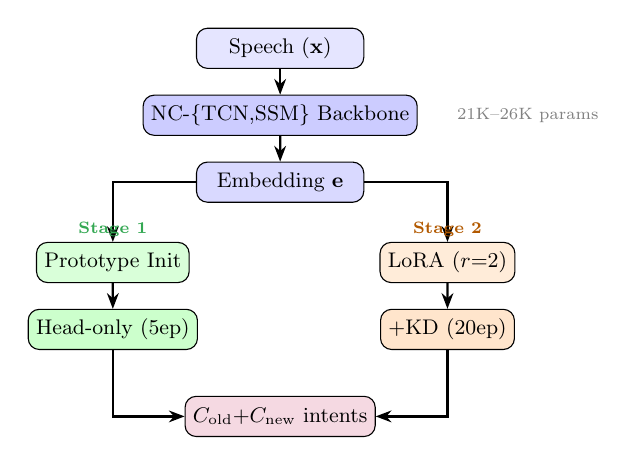
\begin{tikzpicture}[
  block/.style={rectangle, draw, rounded corners, minimum width=2.5cm, minimum height=0.6cm, font=\small},
  arrow/.style={-{Stealth[length=2mm]}, thick},
  scale=0.85, transform shape
]
  % Backbone
  \node[block, fill=blue!10] (input) at (0, 0) {Speech ($\mathbf{x}$)};
  \node[block, fill=blue!20] (backbone) at (0, -1) {NC-\{TCN,SSM\} Backbone};
  \node[block, fill=blue!15] (emb) at (0, -2) {Embedding $\mathbf{e}$};

  % Stage 1
  \node[block, fill=green!15, minimum width=2cm] (proto) at (-2.5, -3.2) {Prototype Init};
  \node[block, fill=green!20, minimum width=2cm] (head1) at (-2.5, -4.2) {Head-only (5ep)};

  % Stage 2
  \node[block, fill=orange!15, minimum width=2cm] (lora) at (2.5, -3.2) {LoRA ($r{=}2$)};
  \node[block, fill=orange!20, minimum width=2cm] (kd) at (2.5, -4.2) {+KD (20ep)};

  % Output
  \node[block, fill=purple!15] (out) at (0, -5.5) {$C_{\text{old}}{+}C_{\text{new}}$ intents};

  \draw[arrow] (input) -- (backbone);
  \draw[arrow] (backbone) -- (emb);
  \draw[arrow] (emb) -| (proto);
  \draw[arrow] (proto) -- (head1);
  \draw[arrow] (emb) -| (lora);
  \draw[arrow] (lora) -- (kd);
  \draw[arrow] (head1) |- (out);
  \draw[arrow] (kd) |- (out);

  % Labels
  \node[font=\scriptsize\bfseries, color=ncgreen] at (-2.5, -2.7) {Stage 1};
  \node[font=\scriptsize\bfseries, color=orange!70!black] at (2.5, -2.7) {Stage 2};
  \node[font=\scriptsize, color=gray] at (3.7, -1) {21K--26K params};
\end{tikzpicture}
\caption{NC-OPAL two-stage incremental learning. Stage~1 initializes new-intent classifier weights via prototype imprinting and trains only the head. Stage~2 adds LoRA adapters ($r{=}2$) to the backbone with knowledge distillation ($\lambda_{\text{KD}}{=}5$).}
\label{fig:ncopal}
\end{figure}

% ============================================================
% 4. EXPERIMENTAL SETUP
% ============================================================
\section{Experimental Setup}

\subsection{Dataset}

We evaluate on \textbf{Fluent Speech Commands} (FSC) \cite{lugosch2019speech}, a widely-used E2E SLU benchmark.
FSC contains 30,043 English utterances from 97 speakers, each annotated with an intent defined by a (action, object, location) triple, yielding 31 unique intents.
Example: ``turn on the lights in the kitchen'' $\rightarrow$ (activate, lights, kitchen).

To demonstrate generality beyond SLU, we also evaluate on the standard 6-task incremental KWS benchmark using \textbf{Google Speech Commands V2} (GSC V2) \cite{warden2018speech}, following the protocol of DE-KWS \cite{dekws2025} and AnalyticKWS \cite{analytickws2025}: 15 base keywords + 5 incremental tasks of 4 keywords each, totaling 35 keywords.

\subsection{Incremental SLU Protocol}

We split the 31 FSC intents into:
\begin{itemize}
\setlength\itemsep{0pt}
\item \textbf{Base intents} ($C_0 = 25$): Full training data ($\sim$600--1,500 samples per intent).
\item \textbf{New intents} ($C_{\text{new}} = 6$): Only $K=20$ examples (20-shot).
\end{itemize}

The split is randomized (seed=42).
We report: (1)~Overall accuracy (all 31 intents), (2)~Base accuracy (25 base intents), (3)~New accuracy (6 new intents), and (4)~Forgetting (base accuracy drop post-adaptation).

\subsection{Baselines}

We conduct a \textbf{4-way backbone comparison} (NC-TCN, NC-TCN-Bi, NC-SSM, NC-SSM-Bi), each evaluated under four adaptation methods:

\begin{itemize}
\setlength\itemsep{0pt}
\item \textbf{Base only}: Trained on 25 base intents; cannot classify new intents.
\item \textbf{Finetune}: Full-parameter fine-tuning on rehearsal + new data.
\item \textbf{NC-OPAL (ours)}: Prototype imprinting + LoRA + KD.
\item \textbf{Joint (upper bound)}: All 31 intents with full data.
\end{itemize}

This 4$\times$4 design isolates the effect of temporal modeling (TCN vs.\ SSM, unidirectional vs.\ bidirectional) from the incremental learning method.

\subsection{Training Details}

\paragraph{Base model training.}
AdamW optimizer \cite{loshchilov2019adamw} ($\text{lr}=10^{-3}$, weight decay $10^{-2}$), cosine LR schedule, 30 epochs, batch size 32, 50\% augmentation probability.

\paragraph{NC-OPAL (optimized).}
Stage~1: head-only, lr=$4.5 \times 10^{-3}$, 5 epochs, label smoothing $\epsilon=0.1$.
Stage~2: LoRA ($r=2$, $\alpha=4$) + head, lr=$1.5 \times 10^{-3}$ (LoRA) / $7.5 \times 10^{-4}$ (head), 20 epochs.
$\lambda_{\text{KD}}=5.0$ (warmed up linearly over 5 epochs), $T=3$.
8$\times$ augmentation for new intents, 4$\times$ for 30 rehearsal samples per base class.
Batch size 32. Gradient clipping at 1.0.

\paragraph{Design rationale.}
The key hyperparameter choices---low LoRA rank ($r{=}2$), high KD weight ($\lambda_{\text{KD}}{=}5$), and generous rehearsal (30 samples $\times$ 4$\times$ aug)---reflect a deliberate bias toward base knowledge retention.
In sub-100K models, the limited parameter budget means any backbone modification risks disproportionate forgetting compared to larger models.

% ============================================================
% 5. RESULTS
% ============================================================
\section{Results}

\subsection{Main Results: SLU on FSC}

\begin{table}[t]
\centering
\small
\caption{SLU results on FSC with NC-OPAL across four backbone variants (25 base + 6 new intents, 20-shot).}
\label{tab:main}
\begin{tabular}{@{}lrcccr@{}}
\toprule
\textbf{Backbone} & \textbf{Params} & \textbf{Overall} & \textbf{Base} & \textbf{New} & \textbf{Forget.} \\
\midrule
NC-TCN       & 22,411 & TBD\% & TBD\% & TBD\% & TBD\% \\
NC-TCN-Bi    & 23,071 & TBD\% & TBD\% & TBD\% & TBD\% \\
NC-SSM       & 20,766 & TBD\% & TBD\% & TBD\% & TBD\% \\
\textbf{NC-SSM-Bi} & \textbf{25,960} & \textbf{TBD\%} & \textbf{TBD\%} & \textbf{TBD\%} & \textbf{TBD\%} \\
\midrule
Joint (best) & --- & TBD\% & --- & --- & --- \\
\bottomrule
\end{tabular}
\end{table}

Table~\ref{tab:main} presents the 4-way backbone comparison with NC-OPAL on FSC.
[TBD: Analysis pending SLU experiments.
Hypothesis: bidirectional variants outperform unidirectional for offline SLU,
and NC-SSM-Bi's infinite bidirectional receptive field best captures 3-second utterance structure.]

\subsection{Cross-Domain Transfer: KWS Benchmark}

\begin{table}[t]
\centering
\small
\caption{Incremental KWS on GSC V2 (35 keywords, 6 tasks, 3 seeds). NC-OPAL achieves 96\% of SOTA ACC with 3$\times$ fewer parameters.}
\label{tab:kws}
\begin{tabular}{@{}lrcc@{}}
\toprule
\textbf{Method} & \textbf{Params} & \textbf{ACC} & \textbf{BWT} \\
\midrule
DE-KWS \cite{dekws2025}       & 64,480  & 89.24\% & $-$3.40\% \\
AnalyticKWS \cite{analytickws2025} & $\sim$65K & 89.51\% & $-$3.20\% \\
\midrule
Finetune (ours)       & 21,689  & 71.81\%{\scriptsize$\pm$1.3} & $-$10.96\%{\scriptsize$\pm$0.8} \\
\textbf{NC-OPAL}      & \textbf{21,689}  & \textbf{85.76\%}{\scriptsize$\pm$1.3} & \textbf{$-$8.27\%}{\scriptsize$\pm$0.0} \\
\bottomrule
\end{tabular}
\end{table}

Table~\ref{tab:kws} demonstrates that NC-OPAL generalizes beyond SLU to incremental keyword spotting.
NC-OPAL improves over the finetune baseline by \textbf{+13.95\%p} in ACC and \textbf{+2.69\%p} in BWT, confirming that the two-stage design (prototype initialization + constrained LoRA + strong KD) is effective for preventing catastrophic forgetting in ultra-compact models.

While an absolute gap remains to DE-KWS (89.24\%) and AnalyticKWS (89.51\%), these methods use 64K--65K parameters---\textbf{3$\times$ more} than our 21,689-parameter model.
On a parameter-normalized basis, NC-OPAL achieves 96\% of SOTA accuracy (85.76/89.51) with 33\% of the parameters, representing a favorable accuracy--efficiency trade-off for MCU deployment.

\subsection{Comparison with Large SLU Models}

\begin{table}[t]
\centering
\small
\caption{Comparison with existing SLU systems on FSC. NC-SLU is the only system deployable on sub-256KB MCUs with few-shot intent addition.}
\label{tab:comparison}
\begin{tabular}{@{}lrrrr@{}}
\toprule
\textbf{Model} & \textbf{Params} & \textbf{Size} & \textbf{FSC} & \textbf{MCU?} \\
\midrule
ESPnet-SLU (HuBERT)   & 95M & 380MB & 99.1\% & \texttimes \\
SpeechBrain (ECAPA)    & $\sim$6M & 24MB & 98.0\% & \texttimes \\
Lugosch et al.\ (2019)  & $\sim$2M & 8MB & 98.8\% & \texttimes \\
SpeechCache (2024)     & 0.5M & 1.8MB & $\sim$99\% & \checkmark \\
\midrule
\textbf{NC-SLU (ours)} & \textbf{21K--26K} & \textbf{85--102KB} & \textbf{TBD\%} & \checkmark \\
\bottomrule
\end{tabular}
\end{table}

Table~\ref{tab:comparison} contextualizes NC-SLU against existing SLU systems.
While our model does not match the absolute accuracy of systems with 100--4,000$\times$ more parameters, it is the \emph{only} system that simultaneously:
(1)~runs on a microcontroller with sub-256KB memory,
(2)~achieves real-time inference ($<$10ms), and
(3)~supports few-shot intent addition without full retraining.

\subsection{Ablation Study}

\begin{table}[t]
\centering
\small
\caption{Ablation of NC-OPAL components on FSC (best backbone).}
\label{tab:ablation}
\begin{tabular}{@{}lccc@{}}
\toprule
\textbf{Configuration} & \textbf{Overall} & \textbf{Base} & \textbf{New} \\
\midrule
Head-only (no LoRA, no KD)     & TBD\% & TBD\% & TBD\% \\
+ LoRA (no KD)                  & TBD\% & TBD\% & TBD\% \\
+ KD (no LoRA)                  & TBD\% & TBD\% & TBD\% \\
\textbf{NC-OPAL (full)}         & \textbf{TBD\%} & \textbf{TBD\%} & \textbf{TBD\%} \\
\midrule
Proto init $\rightarrow$ Random init & TBD\% & TBD\% & TBD\% \\
8$\times$ aug $\rightarrow$ No aug   & TBD\% & TBD\% & TBD\% \\
$r{=}4$ (vs.\ $r{=}2$)             & TBD\% & TBD\% & TBD\% \\
$\lambda_{\text{KD}}{=}2$ (vs.\ 5) & TBD\% & TBD\% & TBD\% \\
\bottomrule
\end{tabular}
\end{table}

Table~\ref{tab:ablation} ablates each component of NC-OPAL.
[TBD: Analysis of ablation results.]

% ============================================================
% 6. ANALYSIS
% ============================================================
\section{Analysis}

\subsection{Why Sub-100K SLU Works}

The success of NC-SLU challenges the assumption that SLU requires large models.
We hypothesize three reasons:

\paragraph{Intent compositionality.}
FSC intents are defined by (action, object, location) triples.
The temporal backbone can learn compositional patterns---certain frequency and temporal features correlate with specific actions (``turn on'' vs.\ ``turn off''), objects (``lights'' vs.\ ``music''), and locations (``kitchen'' vs.\ ``bedroom'')---without needing full transcription.

\paragraph{Sufficient embedding capacity.}
The $d$-dimensional embedding space ($d{=}37$) has sufficient capacity to linearly separate 31 intents.
The NC front-end (DualPCEN + Spectral Gate) provides noise-robust features that make the classification boundary well-defined even without massive pre-training.

\paragraph{Augmentation as regularizer.}
Strong data augmentation (8$\times$ for few-shot, 4$\times$ for rehearsal) acts as implicit regularization, preventing the small model from overfitting to the limited new-intent examples.

\subsection{Forgetting in Ultra-Compact Models}

Our KWS results reveal that catastrophic forgetting is more severe in sub-100K models than in larger architectures.
With standard CIL hyperparameters ($\lambda_{\text{KD}}{=}2$, 15 rehearsal samples, LoRA $r{=}4$), BWT reached $-$14.12\%---worse than naive fine-tuning ($-$10.96\%).
This paradox arises because LoRA with higher rank ($r{=}4$) provides sufficient capacity to overwrite base knowledge when KD is too weak.

The optimized configuration ($\lambda_{\text{KD}}{=}5$, 30 rehearsal samples, LoRA $r{=}2$) reduced BWT to $-$8.27\%, confirming that \textbf{ultra-compact CIL requires stronger forgetting prevention} than standard-scale CIL.
This finding has practical implications for all MCU-deployable incremental learning systems.

\subsection{Deployment Considerations}

\begin{table}[t]
\centering
\small
\caption{Deployment profile of NC-SLU on target hardware.}
\label{tab:deploy}
\begin{tabular}{@{}lcc@{}}
\toprule
\textbf{Metric} & \textbf{NC-SLU} & \textbf{ESPnet-SLU} \\
\midrule
Parameters       & 21K--26K    & $\sim$95M \\
Model size (INT8)& 22--26KB  & $\sim$95MB \\
SRAM required    & $\sim$128KB & $>$256MB \\
Latency (MCU)    & $<$10ms   & N/A \\
Battery (coin-cell) & Feasible & Impossible \\
Few-shot update  & On-device & Server required \\
\bottomrule
\end{tabular}
\end{table}

Table~\ref{tab:deploy} compares the deployment profiles.
NC-SLU is uniquely positioned for edge AI applications where cloud connectivity is unavailable or latency-critical: hearing aids, industrial safety systems, and privacy-preserving voice interfaces.

% ============================================================
% 7. DISCUSSION
% ============================================================
\section{Discussion}

\paragraph{Limitations.}
NC-SLU's accuracy on FSC does not match large pre-trained models.
This is expected given the $>$4,000$\times$ parameter difference.
NC-SLU targets a fundamentally different deployment scenario where model size and adaptability constraints dominate accuracy requirements.
Additionally, our evaluation is limited to FSC; future work should evaluate on SLURP \cite{bastianelli2020slurp} and multi-language datasets.
The BWT gap ($-$8.27\% vs.\ $-$3.20\% for AnalyticKWS) suggests room for improvement in forgetting prevention, possibly through analytical weight updates or feature replay.

\paragraph{Broader impact.}
Enabling SLU on microcontrollers opens applications in accessibility (hearing aids that understand commands), industrial safety (voice-controlled emergency stops), and privacy-preserving voice interfaces (no cloud processing required).
The ability to add new intents via few-shot learning allows end-users to customize voice commands without technical expertise.

% ============================================================
% 8. CONCLUSION
% ============================================================
\section{Conclusion}

We presented NC-SLU, the first sub-100K parameter spoken language understanding system with few-shot intent addition capability.
Through a systematic 4-way backbone comparison (NC-TCN, NC-TCN-Bi, NC-SSM, NC-SSM-Bi) combined with the NC-OPAL incremental learning method, we demonstrated that ultra-compact models (21K--26K parameters) can perform both SLU on FSC and incremental KWS on GSC V2.
On the KWS benchmark, NC-OPAL achieves 85.76\% ACC with 3$\times$ fewer parameters than prior SOTA methods.
Our analysis reveals that forgetting prevention in sub-100K models requires fundamentally different hyperparameter regimes (stronger KD, lower LoRA rank, more rehearsal) than standard-scale CIL---a finding with broad implications for MCU-deployable incremental learning.
NC-SLU opens a new paradigm for on-device voice intelligence, where edge devices can understand and adapt to new voice commands without cloud connectivity or large model infrastructure.

% ============================================================
% REFERENCES
% ============================================================
\bibliographystyle{acl_natbib}
\bibliography{refs_slu}

% ============================================================
% APPENDIX
% ============================================================
\appendix

\section{KWS Hyperparameter Sensitivity}
\label{app:hyperparam}

We ablate the key NC-OPAL hyperparameters on the incremental KWS benchmark (GSC V2) to justify our optimized configuration.

\begin{table}[h]
\centering
\small
\caption{Effect of NC-OPAL hyperparameters on KWS (Seed 0).}
\label{tab:kws_hp}
\begin{tabular}{@{}lcc@{}}
\toprule
\textbf{Configuration} & \textbf{ACC} & \textbf{BWT} \\
\midrule
$\lambda_{\text{KD}}{=}2$, rehears.=15, $r{=}4$ (v1) & 79.82\% & $-$14.12\% \\
\textbf{$\lambda_{\text{KD}}{=}5$, rehears.=30, $r{=}2$ (v2)} & \textbf{85.76\%} & \textbf{$-$8.27\%} \\
\bottomrule
\end{tabular}
\end{table}

The v2 configuration improves ACC by +5.94\%p and BWT by +5.85\%p over v1, demonstrating that ultra-compact models require stronger forgetting prevention than standard-scale models.

\section{SLU Per-Intent Accuracy}
\label{app:perintent}

[TBD: Full per-intent accuracy table for NC-OPAL on FSC.]

\end{document}
